\begin{savequote}[75mm]
I rarely find it useful to distinguish between theory and practice; their interplay is already profound and will only increase as the systems and problems we consider grow more complex.
\qauthor{Michael I. Jordan}
\end{savequote}

\chapter{A Web Implementation of the Luna Rating System}

\section{Introduction}

The Luna Rating System is designed to be a practical test for machine intelligence. It may offer some utility as a thought experiment, but its primary value can only be realized in practice. In this chapter, I describe the design and launch of the first web-based implementation of LRS. The application is meant to serve as a comprehensive proof-of-concept. For the application to fulfill its purpose, it must first be capable of recruiting and handling hundreds of human players. The design should then persuade players to play several games, so as to refine their Smarts Ratings. Finally, the behavior of players should indicate a collective understanding of the Luna Game, and evidence should suggest their aspirations towards honest play.

The baseline success of the LRS implementation can be easily measured through traffic statistics: how many players play, and how long do they typically stay? Such statistics comprise the first section of results in this chapter. In addition to these standard metrics, the questions and responses traded by the players can be assessed qualitatively. I provide a representative sample of questions and discuss common themes from the full dataset. The final source of results is derived from human players' interactions with simple standardized machine players. I argue that the Guesses that human players make of the machine players should converge over time as a consensus on the semantics of Smarts Ratings is reached. Machine players also provide a demonstration for AI researchers who wish to introduce their own machines into the system.

\section{Building the Web Interface}

\subsection{Design of the Web Interface}

My implementation of the Luna Rating System is built on the open-source software stack consisting of MongoDB, Express.js, Angular.js, and Node.js, which is collectively referred to as the MEAN stack \citep{karpov2013mean}. The latter three technologies are all written in JavaScript and MongoDB is a NoSQL database. At a very high level, MongoDB stores all player and game data, Angular.js controls and displays the client side, Express.js forms the foundation of the server side, and Node.js runs the code written on top of that foundation. Notable libraries used include: Mongoose.js, a Node.js library for interfacing with MongoDB; Passport.js, a Node.js library which provides middleware for user authentication; and Angular-UI, an Angular.js library that simplifies routing, i.e. navigation between different states of the website. The front end of the website, i.e. the style, formatting, and organization of content, was modified from the ``Material Admin'' LESS/Angular.js template, for which I purchased a single application license. The site was developed locally and then hosted on EC2 by Amazon Web Services under the domain name \url{luna-game.com}.

The website's wireframe layout was first prototyped on paper, which allowed for iteration on the skeletal design \citep{rettig1994prototyping}. The centerpiece of the website is the ongoing Luna Games, and a secondary component allows users to review their performance in previous Games. To reduce user drop-off, the front end seamlessly leads a user between the phases of a Luna Game within a single page. All opportunities for latency --- between phases of a Game or between Games ---  are reduced as much as possible to encourage repeated play. To increase the probability that a first-time user explores the website beyond the landing page, the website has an option to play as a ``guest.'' The only functional difference between a user that signs up and a guest is that signed up users may log out and log back in, while a guest account expires once the $60$-day token is removed from the browser or the user explicitly signs out. Further consideration was given to user experience in the context of the results presented in Chapter $3$ of this thesis, which demonstrate that all players must have a clear understanding of their goals during a Luna Game. While it is important that users be able to start playing Luna Games as quickly as possible, they should first be fully aware of the Game's structure and their goals.

Weighing these considerations, the core features of the website are divided into $10$ primary states and $4$ secondary states. The secondary states include static pages --- the contact page and two extended information pages --- and one profile page that allows a user to review statistics related to her historical performance. The primary states are presented in Figure \ref{statediagram}. They include four states corresponding to the phases of a Luna Game, one home state, which contains games as nested states, a landing page, a guest state, a sign up state, a login state, and an information state. Note that first-time users must provide consent and review information about the structure of Luna Games before they are able to play. The eager first-time user is able to reach a new game with only three clicks from the home page, and a returning user can reach games with two clicks and a form submission. This simple state architecture ensures that users are well-informed of the rules and then playing as soon as possible. Screenshots of a typical user experience are depicted in Figure \ref{screenshotpic}.

\begin{figure}
\begin{scriptsize}
\begin{center}
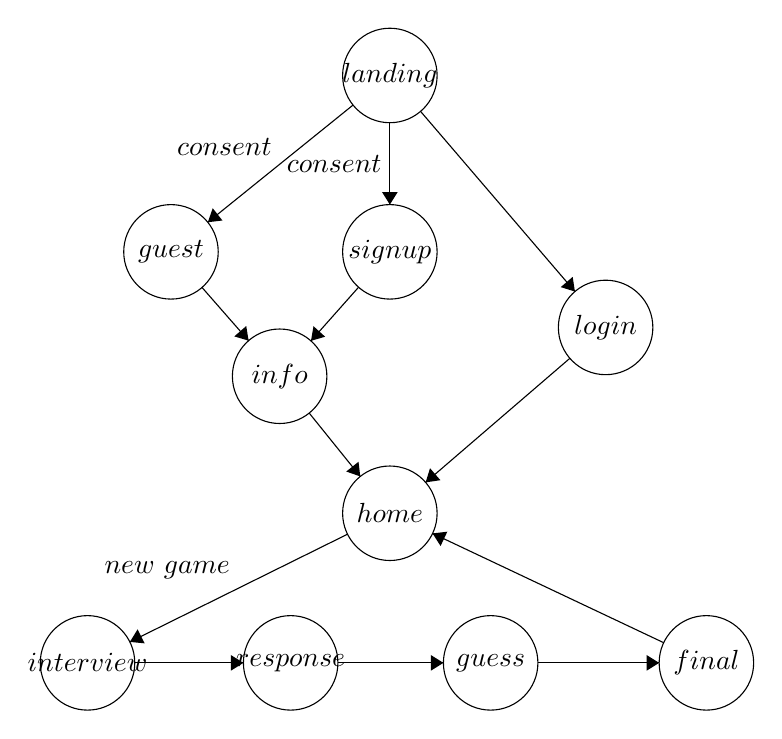
\begin{tikzpicture}[scale=0.2]
\tikzstyle{every node}+=[inner sep=0pt]
\draw [black] (38.9,-3.4) circle (3);
\draw (38.9,-3.4) node {$landing$};
\draw [black] (25,-14.6) circle (3);
\draw (25,-14.6) node {$guest$};
\draw [black] (38.9,-14.6) circle (3);
\draw (38.9,-14.6) node {$signup$};
\draw [black] (52.6,-19.4) circle (3);
\draw (52.6,-19.4) node {$login$};
\draw [black] (38.9,-31.2) circle (3);
\draw (38.9,-31.2) node {$home$};
\draw [black] (19.7,-40.7) circle (3);
\draw (19.7,-40.7) node {$interview$};
\draw [black] (32.6,-40.7) circle (3);
\draw (32.6,-40.7) node {$response$};
\draw [black] (45.3,-40.7) circle (3);
\draw (45.3,-40.7) node {$guess$};
\draw [black] (59,-40.7) circle (3);
\draw (59,-40.7) node {$final$};
\draw [black] (31.9,-22.5) circle (3);
\draw (31.9,-22.5) node {$info$};
\draw [black] (38.9,-6.4) -- (38.9,-11.6);
\fill [black] (38.9,-11.6) -- (39.4,-10.8) -- (38.4,-10.8);
\draw (38.4,-9) node [left] {$consent$};
\draw [black] (36.56,-5.28) -- (27.34,-12.72);
\fill [black] (27.34,-12.72) -- (28.27,-12.61) -- (27.65,-11.83);
\draw (28.39,-8.51) node [above] {$consent$};
\draw [black] (40.85,-5.68) -- (50.65,-17.12);
\fill [black] (50.65,-17.12) -- (50.51,-16.19) -- (49.75,-16.84);
\draw [black] (50.33,-21.36) -- (41.17,-29.24);
\fill [black] (41.17,-29.24) -- (42.11,-29.1) -- (41.45,-28.34);
\draw [black] (36.21,-32.53) -- (22.39,-39.37);
\fill [black] (22.39,-39.37) -- (23.33,-39.46) -- (22.88,-38.57);
\draw (24.76,-35.43) node [above] {$new\mbox{ }game$};
\draw [black] (22.7,-40.7) -- (29.6,-40.7);
\fill [black] (29.6,-40.7) -- (28.8,-40.2) -- (28.8,-41.2);
\draw [black] (35.6,-40.7) -- (42.3,-40.7);
\fill [black] (42.3,-40.7) -- (41.5,-40.2) -- (41.5,-41.2);
\draw [black] (48.3,-40.7) -- (56,-40.7);
\fill [black] (56,-40.7) -- (55.2,-40.2) -- (55.2,-41.2);
\draw [black] (56.29,-39.42) -- (41.61,-32.48);
\fill [black] (41.61,-32.48) -- (42.12,-33.28) -- (42.55,-32.37);
\draw [black] (33.78,-24.84) -- (37.02,-28.86);
\fill [black] (37.02,-28.86) -- (36.91,-27.93) -- (36.13,-28.55);
\draw [black] (26.97,-16.86) -- (29.93,-20.24);
\fill [black] (29.93,-20.24) -- (29.78,-19.31) -- (29.02,-19.97);
\draw [black] (36.91,-16.85) -- (33.89,-20.25);
\fill [black] (33.89,-20.25) -- (34.79,-19.99) -- (34.05,-19.32);
\end{tikzpicture}
\end{center}
\end{scriptsize}
\caption{Schematic diagram depicting the primary states of the Luna Rating System web interface. Nodes represent website states and edges indicate how users typically navigate between states. A first-time user arrives at the \textit{landing} state. Upon providing consent, the user may play as a \textit{guest} or \textit{sign up}, both which lead to the \textit{info} state. The info state explains the Luna Game and then directs users to the \textit{home} state. The user can then create a new Luna Game, launching the \textit{interview} state. As the user progresses through the Luna Game, she transitions from interview to \textit{response}, to \textit{guess}, and to \textit{final}. They then return to the home state to start another game. Returning signed up users may \textit{login} from the landing state to reach the home state.}
\label{statediagram}
\end{figure}

\begin{figure}
\includegraphics[width=0.5\textwidth]{figures/screen1.png}
\includegraphics[width=0.5\textwidth]{figures/screen2.png}
\includegraphics[width=0.5\textwidth]{figures/screen3.png}
\includegraphics[width=0.5\textwidth]{figures/screen4.png}
\includegraphics[width=0.5\textwidth]{figures/screen5.png}
\includegraphics[width=0.5\textwidth]{figures/screen6.png}
\caption{Exemplary screenshots of the Luna website. Clockwise from top left: the landing page, the information page for first-time users, interview phase, response phase, guess phase, and final phase.}
\label{screenshotpic}
\end{figure}

\subsection{An API for Machine Players}

To allow AI researchers to enter machines as players on the Luna Rating System website, I implemented a RESTful API. Machine players must first register separately from human players to receive an API token. This process is currently done by hand, since the system is not yet protected against malicious machine players (e.g. there is no limit on the number of API calls that one player may make). The experience of machine players is very similar to that of humans. The machine may make a request to start a new game, provide questions during the interview phase of an ongoing game, receive questions and provide answers during the response phase, provide a guess during the guess phase, and receive any updates of its own Smarts Rating and total wins. Notably, the guess of a machine is not factored into the Smarts Rating of its opponent. A Python template, which may be used directly or as a blueprint for other languages, is provided for researchers. 


This study implemented two simple machine players, both of which were equipped with a fixed set of $5$ questions to present during all Interview Phases for consistency. The questions were:

\begin{enumerate}
\item What color is the sky?
\item What is the direct object in this sentence: ``The boy threw the ball to the dog''? 
\item Why is $6$ afraid of $7$?
\item Why does poverty exist?
\item What is the capital of New York?
\end{enumerate}

The only distinction between the two machines was their response functions. The first machine, which I refer to as the Gibberish Bot, responds to any question by generating a random string of uppercase characters, digits, and spaces. The length of the response is also randomly selected to be between $1$ and $200$. This machine is meant to serve as the most basic of controls; if Smarts Ratings are at all meaningful, the Gibberish Bot should have a very low one. The second machine, referred to as the Cleverbot, responds to questions by querying the Cleverbot chatbot, a web-based chatbot that responds to human inputs by outputting previously seen human inputs that are deemed most similar according to a simple surface-level analysis  \citep{carpenter2015cleverbot}. Cleverbot is an ideal second control, as it provides responses that have been written by humans, but does not attempt to understand these questions with any level of sophistication. Thus one would reasonably expect Cleverbot to achieve a Smarts Rating higher than the Gibberish Bot, but lower than most humans. Each bot played $9$ games, alternating one at a time against randomly selected human opponents in the first few days of the launch.

\subsection{Launching the Website}

Since this work relies on human participation, the study was submitted for review to the Committee on the Use of Human Subjects in Research at Harvard University. The study qualified for expedited review and received approval on February $18$, $2016$. The website was immediately launched and publicized, primarily via social media and email. Publicity efforts continued for one week following the launch. The results presented in this chapter were gathered in the two weeks following launch, up until March $3$, $2016$. 

\section{Results}

\subsection{Traffic Summary}

In the first two weeks of the Luna web implementation, the site attracted $1293$ registered players (including the two machine players). $685$ Luna Games were initiated, creating $4173$ unique questions and $4923$ responses. According to Google Analytics, the website earned $2312$ sessions and $2937$ page views. Slightly over $30$\% of visitors were returning to the site. $54$\% of the visitors came to the site directly, e.g. through clicking a link in their email or typing the URL manually, while the remaining visitors were referred primarily through Facebook and Twitter. The daily number of sessions is plotted in Figure \ref{trafficplot}. As expected, the amount of traffic correlates strongly with publicity efforts, which were concentrated in the first few days of the launch and virtually ceased after one week.

\begin{figure}
\includegraphics[width=0.95\textwidth]{figures/trafficPlot.png}
\caption{Daily traffic to the Luna web implementation in the first two weeks after launch. Publicity for the site was concentrated in the first few days of the launch and virtually ceased after one week.}
\label{trafficplot}
\end{figure}

\subsection{Human Player Summary}

The vast majority of human players registered as guests ($1207$), while very few ($86$) signed up using their emails. One consequence of this discrepancy is that only a small fraction of users were able to receive email updates when it was their turn to play in a Luna Game. In addition, many users appear to have registered as guests and then left the site without submitting interview questions; the overall average number of games played was $0.33$, with a median of $0$. This is not to say that the guest registration option was ill-advised; it is likely that removing the guest option would have yielded far fewer registrations overall. However, anecdotal evidence suggests that the frequent stalling of Luna Games, due to guests leaving in the middle of a Game, led to frustration among more dedicated players. Among the $220$ players who did complete at least one full game, the average Smarts Rating was $68.9$, with a median of $74$. The full distribution of Smarts Ratings for human players is depicted in Figure \ref{humansmartsratings}. The ratings exhibit a bell curve roughly around the mean with a few low outliers. 

%In Figure \ref{smartsratingscorrelation}, I consider whether Smarts Ratings are correlated with the number of games played or won. 

\begin{figure}
\includegraphics[width=0.95\textwidth]{figures/ratingDistribution.png}
\caption{\label{humansmartsratings} Smarts Rating distribution of human players who completed at least one full Luna Game. The ratings exhibit a bell curve roughly around the mean of $68.9$ with a few low outliers.}
\end{figure}

\subsubsection{Sample Questions and Responses}

I plan to publicly release the complete dataset of questions and responses through the Harvard Dataverse Network after the submission of this thesis. The below $10$ examples are meant to be representative of the full dataset in terms of question and response length, form, and content.

\begin{enumerate}

\item Q: Is addiction a disease, as is increasingly being claimed, or is the addict at fault for developing their addiction?
\\ A: a bit of each; people can be psychologically and/or genetically liable to develop addictions, but with sufficient willpower they needn't

\item Q: Apparently, our senses can detect around $11$ million pieces of information per second. How much total can a human process of this $11$ million? A: $10$ of those B: all $11$ million C: $25$ to $30$ of those D: $5$ to $7$ of those
\\ A: B

\item Q: Compose a limerick involving the word jello.
\\ A: hey there fellow; I hate jello; it's not tasty; I'm being hasty; hard question, well-oh...

\item Q: What is the biggest risk from self-driving cars?
\\ A: Two things.  First, we currently have no way of integrating self-driving cars into current traffic patterns.  The self-driving cars are better at driving than people are, and a road with only self-driving cars would be much safer and far more efficient, but trying to work around humans will cause all sorts of headaches and loss of efficiency.  For example, there are algorithms for having autonomous cars coordinate at interesections so that they can all drive through a full speed from all directions and never hit each other; if you had to throw even one human-driven car into that mix, then whole system would have to stop.  Second, current cars are disturbingly hackable.  Security researchers have demonstrated over and over that it's super easy to remotely take control of a car, and have the ability to mess with it in all kinds of ways (e.g. disable the breaks), but car companies just don't care and will not implement any security because consumers don't care and it would cost the companies extra money.  Obviously as cars become even more autonomous, this security risk will grow even further.  Sorry, that was really long... but I spend too much time thinking about these things.

\item Q: What causes the McGurk effect?
\\ A: Our brain confuses visual inputs with auditory ones.

\item Q: What is the strangest experience you have ever had while riding a bus?
\\ A: Overhearing a taxidermist telling a random person how much he loved his job and then asking how their pet was doing

\item Q: Who am I?
\\ A: Is a question that usually strikes us with the most weight around the age of $50$.

\item Q: Should Supreme Court positions have term limits?
\\ A: don't understand the question. is this about USA? this game is worldwide.

\item Q: Who is/was the most influencial person in your life?
\\ A: I am

\item Q: Describe an algorithm for walking
\\ A: Brain signal -> knee. $\^$ knee. Increment $37$ degrees. + $1.5$ feet forward. Repeat for other knee.
\end{enumerate}

\subsection{Machine Player Summary}

After $9$ games each, the Gibberish Bot achieved a Smarts Rating of $6.4$, and Cleverbot arrived at a Smarts Rating of $40.4$. All opponents but one guessed a Smarts Rating of 1 for the Gibberish Bot; the remaining opponent guessed $50$. Guesses of Cleverbot's Smarts Rating ranged from $5$ to $88$. To illustrate the typical behavior of each of these machines during the Response phase, I provide representative samples below.

\subsubsection{Gibberish Bot Response Phase Sample}
\begin{enumerate}
\item Q: How old are you?
\\A: WE23 F1MTR4FI7YBT16JYRV8AWEY7ALLLXI3M79 1BSL8G

\item Q: Will your answer to this question be wrong?
\\A: MGKGJNYJYHP4XM2J35TQ BF4GNNERA77Z20ZVULH

\item Q: Is the space L$\^2$ complete?
\\A: DZTYWUKXE4D13B58A823VA8 22ZLZ19FQAGPEMQ

\item Q: What is a contradiction to the CAPM model of financial markets?
\\A: PGIITGJWK0NFBTOT

\item Q: What is a bound on spectral sparsification of complete graphs?
\\A: NS2TEEMRSL91ANNF 4LDK2M5YSI4I1JVU6SV74LUKNVAH
\end{enumerate}
Guess: 1

\subsubsection{Cleverbot Response Phase Sample}
\begin{enumerate}
\item Q: What is your favorite book and please describe it in $3$ words.
\\A: Howl by Allen Ginsberg.

\item Q: What's the best thing you did today?
\\A: The moment that I fell in love was the best thing I have seen. You?

\item Q: What is your favorite number from $1$ to $10$ and why?
\\A: Number $13$ is my favorite number.

\item Q: What is the best machine ever invented?
\\A: Back to the Future is the best movie ever.

\item Q: What is your biggest accomplishment of the last year?
\\A: All the time I HAVEN'T spent talking to you!
\end{enumerate}
Guess: $40$

\subsection{Game Summary}

Among the $685$ initiated Luna Games, $292$ were followed through to the final phase by both players. To see if there is any obvious correlation between the length of responses and the subsequent guess of the Smarts Rating of the responder, I created a scatterplot of response length and subsequent guess (Figure \ref{responseLengthGuess}). The relationship between response length and guess gives a Pearson's $r$ of $0.179$, suggesting a weak positive correlation. One interpretation of this result is that players who put more effort into their responses are rewarded with higher Smarts Ratings.

\begin{figure}
\includegraphics[width=0.95\textwidth]{figures/responseVsGuesses.png}
\caption{\label{responseLengthGuess} Relationship between response length and subsequent guess of the responder's Smarts Rating. Pearson's $r$ is $0.179$, suggesting a weak positive correlation.}
\end{figure}

It is impossible to assess whether Smarts Ratings are accurate without presuming some ground truth about intelligence. However, one encouraging sign would be the convergence of a player's Smarts Rating as she continues to play games. In Figure \ref{smartRatingStds}, I plot the standard deviations of Smarts Ratings per player as a function of the number of games each has completed. No such convergence is yet observed, likely indicating that more playing time is necessary for the system to reach an equilibrium in which most players hold a shared understanding of Smarts Ratings. 

\begin{figure}
\includegraphics[width=0.95\textwidth]{figures/varianceGamesPlayed.png}
\caption{\label{smartRatingStds} Standard deviations of Smarts Ratings per player as a function of number of games completed. Convergence as the number of games increases is not yet observed. Note that the values in the plot are standard deviations, and the error bars are standard deviations (over all players) of standard deviations.}
\end{figure}

\section{Analysis}

The first goal of this chapter --- to demonstrate that a straightforward web implementation of the Luna Rating System can draw players and sustain games --- is readily reached. Given the relatively minor publicity efforts, unaided by any sort of financial expenditures, the substantial traffic to the website within the short time window is very encouraging. The Smarts Ratings reached by both human and machine players are also auspicious. The bell curve observed for humans is consistent with the distribution of IQ, for example. Moreover, the Smarts Ratings of the machines --- $6.4$ for the Gibberish Bot and $40.4$ for Cleverbot --- indicate that the controls were relatively successful. As expected, the Gibberish Bot reached a much lower rating than Cleverbot, and Cleverbot remained significantly lower than the majority of human players. These results corroborate the semantic value of Smarts Ratings and suggest that human players understand the basic notion behind the ratings.

While the machine Smarts Ratings align with expectations, the extent to which ratings can meaningfully distinguish between human players is less clear. The weak correlation between response length and subsequent guess can be interpreted in two ways. Optimistically, one would expect that players who are more dedicated to demonstrating intelligence might write longer responses, thus deserving higher Smarts Ratings. Pessimistically, one could argue that Smarts Ratings are just a measure of response length, rather than intelligence. Future work could distinguish between these interpretations by enforcing a stricter limit on response lengths, or by attempting to correlate Smarts Ratings with other metrics of intelligence like IQ. Additionally, the lack of convergence of Smarts Ratings suggests that more time is needed for the system to reach an equilibrium. Once such convergence is observed, the discriminative power of Smarts Ratings will be more clear.

The qualitative results presented in this chapter, consisting mainly of the questions and responses of human players, are perhaps the most encouraging. The questions exhibit a wide range of form, content, length, and difficulty. Some questions are yes/no, multiple choice, or fill in the blank, while others anticipate lengthy free form responses. Some questions are straightforward trivia or simple and subjective (e.g. ``How are you?''), but many require high levels of understanding and logical reasoning. For example, many questions resemble open-ended prompts that one might expect to see on a standardized writing test (e.g. ``Do schools put too much or too little time into Phys. Ed. classes?''). The subsequent responses to these questions are equally broad. The full dataset offers intriguing insight into how humans define and assess intelligence. Moreover, a machine which is to be called artificially intelligent must be able to adequately answer the collected questions.

\section{Discussion}

The results reported in this chapter demonstrate the promising potential of the Luna Rating System as an active and informative benchmark for AI. The study also highlights critical design considerations for future implementations. Perhaps the most confounding aspect of this web implementation was the prevalence of stalled Luna Games. A game stalls when one of the players leaves the website in the middle of gameplay and does not return. The remaining player is left waiting until the game expires due to inactivity (which currently occurs after $3$ days). While waiting players are welcome to start simultaneous games, it is likely discouraging to see a backlog of unfinished games; the incentive to start a new game diminishes as the expectation that games will be finished decreases. If a player registers with an email address, the likelihood that she will return to games improves, as the system automatically sends an email to notify her when it is her turn to play. Thus a central objective in future design should be to obtain valid email addresses. Other ways to further persuade players to stay and play should also be considered.

The primary question left unanswered in this chapter is: what levels of participation are required for Smarts Ratings to reach an equilibrium? There are two dimensions of participations that likely affect this convergence: total number of players, and duration of play. I suspect that increasing the duration of play, i.e. the number of games played per player, is more important than increasing the number of players. An individual player develops an understanding of Smarts Ratings over time as she finishes games and true Smarts Ratings are revealed. The majority of players in this first web implementation have finished no games at all, meaning that they have no empirical basis from which to infer ratings. It is quite possible that even a much smaller cohort of players, each of whom plays several games, would reach a Smarts Rating equilibrium. Future efforts should be focused on achieving this equilibrium; the informativeness of the Luna Rating System depends on the precision of Smarts Ratings.

In addition to revealing refinements for future Luna web implementations, this chapter presents an intriguing original dataset that alone offers several clear avenues for future work. There is the social psychology angle: how do people assess one another's intelligence in practice? There is the NLP perspective: what linguistics features of responses are correlated with subsequent guesses? Simply grouping the questions and responses thematically may reveal rich trends. All participants have given consent in which they acknowledge that their questions and responses may be released as part of a publicly available dataset. I plan to compile such a dataset and release it through the Harvard Dataverse Network in the hope of enabling others to conduct their own analyses.
